\subsection{第二阶段：非坍缩校准与同先验主动取证}
\label{sec:round2}
\paragraph{保留 V1，单独验证其失效原因。}
第~\ref{sec:method} 节及第 4.1--4.4 节报告原始 V1 研究。本节针对一个具体问题展开：如果校准后仍保留合理的候选机制，过程取证能否重新产生可测量的收益？我们保留 \texttt{eb641c2} 的代码、数据和原始结论，在独立分支预先固定新的压力场景、裁决护栏和 30 组开发配置。V1 与 V2 都在新场景上重新评测；不能把新旧基准的分数直接相减，再将差异全部归因于算法。

\paragraph{机制歧义的构造与统计单位。}
新配置采用 256 个智能体、8 个模拟种子、12 个时间步和 200 组候选机制。预先指定的两组机制为 $(a,b,d)=(.2,.95,.12)$ 与 $(.95,.2,.12)$，注意概率与参与概率的乘积相同。通过逆变换共同随机数耦合，二者生成相同的初始意图。历史活动分别启用候补或转发；组合活动同时启用候补通知触发的八邻居传播级联和强同时间冲突。这对机制的历史轨迹 RMSE 为 0.00000，组合探针及测试事件设计上的轨迹分歧为 0.28094。这是专门构造的交互压力测试，不是从真实行为数据拟合出的社会规律。

开发和测试分别使用 12 个与 24 个独立模拟世界。测试更换世界、过程审计和取证答案，事件设计仍与组合探针相同，因此它验证的是同一设计下的新世界复现，不是超出探针的新组合迁移。区间以整个世界为单位进行配对 bootstrap，保留世界内活动之间的依赖，逐活动另行报告。

\paragraph{校准公式与保留条件。}
在 V1 的历史相容支持集 $\mathcal C$ 上，设 $r_{etc}$ 为式~\eqref{eq:distance} 中的相对种子方差归一化项。V2 采用
\begin{align}
 E_m^{(2)}&=\frac{1}{2\sigma^2}\operatorname{mean}_{e,t,c}
 \frac{(\bar X_{metc}-H_{etc})^2}{r_{etc}}+\lambda\ell_m^{\mathrm{proc}},\\
 \ell_m^{\mathrm{proc}}&=-\frac{1}{|\mathcal O|}\sum_{j\in\mathcal O}
 [y_j\log p_{mj}+(1-y_j)\log(1-p_{mj})],\\
 w_{0m}^{(2)}&\propto\mathbf1[m\in\mathcal C]\exp(-E_m^{(2)}/T),\qquad
 T=\inf\{t\geq1:\,N_{\mathrm{eff}}(w_0(t))\geq8\}.
 \label{eq:v2-calibration}
\end{align}
实现中通过二分求解温度，并留出很小的数值余量。MCAR 缺失标签不贡献对数似然；意图记录中未观测的查看状态仍按 $p_{mj}=a_mb_m I_j$ 边缘化。支持集筛选条件不变。上述平均残差对应最终选中的 V2；搜索也包含最坏活动残差版本。Gibbs 温度可以解释为熵正则强度，但这里直接约束的有效机制数对应二阶 R\'enyi 熵，并非 Shannon 熵。

KEEP 必须同时满足：开发 AUC 比当前最优值下降超过 $10^{-8}$；初始有效机制数至少为 8；初始及预算 16 的过程审计 Brier 均不超过 .195；$R(0)-R(16)$ 的配对 95\% bootstrap 区间下界严格大于零；AUC 比同先验 Random 和 Entropy 均至少低 5\%；快速开发评测不超过 15 秒。每个版本内部的三种策略共用先验、证据池、成本、答案、缺失掩码和后验更新。给定所选证据 $D$，更新为
\begin{equation}
 w_m(D)\propto w_{0m}\exp\!\left\{\tau^{-1}
 \sum_{j\in D\cap\mathcal O}\log p_m(y_j)\right\}.
 \label{eq:v2-update}
\end{equation}
最终配置为 $\sigma=0.008$、$\lambda=8$、$\tau=0.5$，各时间步等权，批量大小为 2，并保留幻想分支条件化。假设答案分支与真实证据更新使用相同温度。由于 $\tau\ne1$，该更新属于广义贝叶斯；原协方差评分在此作为启发式排序使用，不能继续宣称它精确等于温度化后验的预期方差下降，也不增加次模性保证。

\paragraph{冻结后的对照结果。}
30 轮有效实验包含 3 次 KEEP、27 次 REVERT，没有运行失败，最优提交为 \texttt{0d094ec}。在同一新缓存上，V2 的初始有效机制数为 26.45，V1 为 1.01。表~\ref{tab:v2-overview} 给出同基准对照。V2 开发 AUC 为 0.07569，比同先验 Random 和 Entropy 分别低 27.5\% 和 43.2\%。读取测试真值前已冻结算法。测试 Full AUC 为 0.05776，95\% 区间为 [0.04948, 0.06688]；V1 为 0.14389，两者相差 59.9\%。V2 的误差从零证据时的 0.13319 降至预算 16 时的 0.03948，配对改善区间为 [0.08321, 0.10258]。初始和最终测试 Brier 分别为 0.18800 与 0.17438。初始 Brier 实际劣于 V1，只是两者均满足护栏；过程预测的改善发生在取证之后。
\begin{table}[tbp]
\centering\small
\setlength{\tabcolsep}{4pt}
\caption{第二阶段同一高分歧基准上的 V1/V2 对照。Brier 为预算 16 的独立过程审计误差。}\label{tab:v2-overview}
\begin{tabular}{llrrrrr}
\toprule
版本 & 划分 & 有效数 & AUC & B0 误差 & B16 误差 & Brier \\
\midrule
V1 & Dev & 1.01 & 0.14410 & 0.14606 & 0.14003 & 0.18197 \\
V2 & Dev & 26.45 & 0.07569 & 0.13327 & 0.04750 & 0.17416 \\
V1 & Test & 1.01 & 0.14389 & 0.14601 & 0.14007 & 0.18223 \\
V2 & Test & 26.45 & 0.05776 & 0.13319 & 0.03948 & 0.17438 \\
\bottomrule
\end{tabular}
\end{table}

\begin{table}[tbp]
\centering\small
\setlength{\tabcolsep}{4pt}
\caption{冻结测试：每个版本内严格共用先验和更新规则，区间按 24 个完整世界重采样。}\label{tab:v2-selectors}
\begin{tabular}{llrlr}
\toprule
版本 & 策略 & AUC & 95\% 区间 & Brier \\
\midrule
V1 & Full & 0.14389 & [0.14281, 0.14474] & 0.18223 \\
V1 & Random & 0.14589 & [0.14561, 0.14618] & 0.18291 \\
V1 & Entropy & 0.14601 & [0.14572, 0.14631] & 0.18296 \\
V1 & ParamIG & 0.14389 & [0.14281, 0.14474] & 0.18223 \\
V1 & Standard\_OED & 0.14392 & [0.14284, 0.14477] & 0.18223 \\
V2 & Full & 0.05776 & [0.04948, 0.06688] & 0.17438 \\
V2 & Random & 0.11579 & [0.10012, 0.13205] & 0.18523 \\
V2 & Entropy & 0.13319 & [0.13294, 0.13346] & 0.18800 \\
V2 & ParamIG & 0.05776 & [0.04948, 0.06688] & 0.17438 \\
V2 & Standard\_OED & 0.13315 & [0.13253, 0.13372] & 0.18810 \\
\bottomrule
\end{tabular}
\end{table}


测试集上，Full AUC 比同先验 Random 低 50.1\%，比同先验 Entropy 低 56.6\%；“基线减 Full”的配对 AUC 差值区间分别为 [0.03946, 0.07722] 与 [0.06633, 0.08376]。图~\ref{fig:v2-curves} 展示逐活动曲线，表~\ref{tab:v2-activities} 给出各活动的区间。然而 ParamIG 选择了相同记录，与 Full 完全持平，因此不能据此声称协方差取证优于参数信息增益。标准 OED 对照针对历史轨迹，表现较弱；它并不是经过优化的组合预测 OED 上界。
\begin{figure}[tbp]
\centering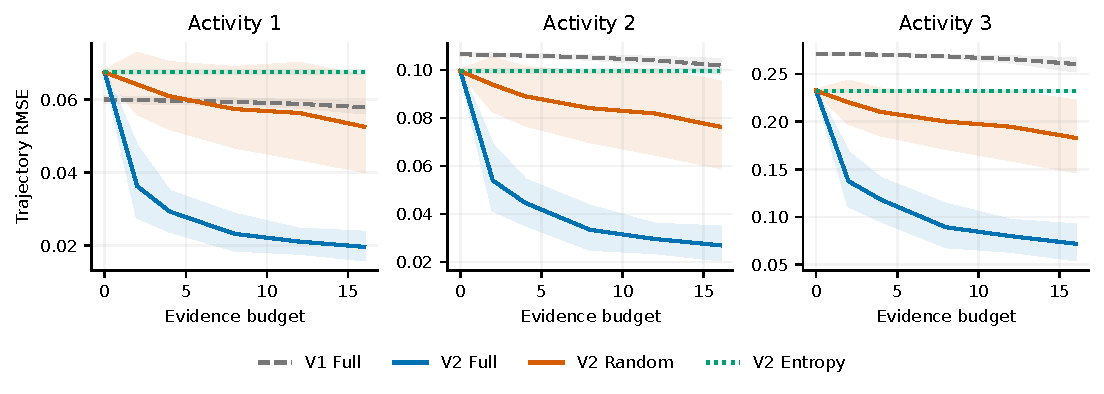
\includegraphics[width=\linewidth]{v2_budget_curves.pdf}
\caption{第二阶段冻结测试的逐活动曲线。阴影为逐点的 95\% 世界 bootstrap 区间。V2 的三种取证共用先验与更新；V1 使用原始校准。ParamIG 与 V2 Full 重合，为便于阅读省略。}
\label{fig:v2-curves}
\end{figure}
\begin{table}[tbp]
\centering\small
\setlength{\tabcolsep}{4pt}
\caption{逐活动的冻结测试结果。每个活动模板有 24 个独立世界实现；同一世界内的活动不视为独立。}\label{tab:v2-activities}
\begin{tabular}{llrll}
\toprule
版本 & 活动 & AUC & AUC 的 95\% 区间 & B0--B16 的 95\% 区间 \\
\midrule
V1 & 1 & 0.05911 & [0.05831, 0.05992] & [0.00109, 0.00358] \\
V1 & 2 & 0.10486 & [0.10382, 0.10567] & [0.00228, 0.00785] \\
V1 & 3 & 0.26770 & [0.26578, 0.26916] & [0.00519, 0.01849] \\
V2 & 1 & 0.02769 & [0.02393, 0.03177] & [0.04375, 0.05123] \\
V2 & 2 & 0.04041 & [0.03429, 0.04726] & [0.06506, 0.07858] \\
V2 & 3 & 0.10519 & [0.09004, 0.12190] & [0.14057, 0.17774] \\
\bottomrule
\end{tabular}
\end{table}


\paragraph{哪些变化有效，哪些结论仍不成立。}
30 组配置产生了 18 个不同的开发 AUC。在最终核宽下，将有效机制数下限从 8 提高到 24 没有改变权重，因为未触发温度提升时的有效机制数已超过 24。因此，护栏可以拒绝不合格候选，但最终配置的改善不能全部归因于护栏主动抬高温度。在核宽 .008、过程权重 8 不变时，将更新温度从 1 调到 .5，AUC 从 0.08193 降至 0.07569；温度 2 则恶化到 0.09056。这是可直接比较的温度实验。其他配置组同时改变核宽、过程权重或损失聚合方式，不能据此单独确定每个因素的因果贡献。移除批量幻想分支条件化后，匹配配置的选择记录和分数相同，这个证据池没有展示独立的批量去冗余收益。

证据池固定包含 24 条查看记录、40 条概率已知为 .5 的可用性记录，以及 96 条边缘化意图记录。最大熵策略将预算花在不可约的可用性随机性上，查看记录则能区分歧义的注意机制。这种设计使失效原因容易解释，也限定了结论：它有利于具有信息敏感性的选择策略，不能证明任意证据池上的普遍优势。测试增益大于开发增益，与固定历史条件下不同的取证答案有关，开发集仅含 12 个世界。当前证据支持“构造场景中恢复了主动取证价值”，尚不支持真实世界机制识别、新的未知规则告警保证或任何官方榜单成绩。
